\section{Edit Based Suggestions For Learning}
\label{sec:edit}
Generating test data using correct queries provided by the instructor works great for finding student queries with errors. However, once the query is found to be incorrect, the student should be awarded partial marks based on the extent of correctness. It is also useful to make suggestions to the students so that can understand the errors in their queries. 

One way to award marks for correctness could have been to use the fraction of datasets (generated by XData) that the student query could pass. This approach turns out to be unfair and could penalize small errors heavily while providing a better score to queries that have more errors. Such examples are shown in \cite{xdata:comad}. Another way to grade student queries would be to just check for the differences between the correct query and the student query. However, this approach may deduct more marks than required as explained below.

\subsection{Approach}


The approach we use instead in XData is to compare the student query to each correct query and make changes or edits to the student query to attempt to make it equivalent to the correct query. After each edit, the student query is compared to the correct query  and the changes are stopped once the student query is equivalent to the correct query. 
Checking for equivalence after each edit could have been done using test data generation but that would be very expensive and grading each student query could take minutes. Other approaches for checking equivalence such as Cosette~\cite{cosette} as well as techniques based on tableau~\cite{tableaux1} work on a limited subset of query constructs and were hence not considered.

Marks are deducted based on the required edits. The edits required are also used to suggest what changes the students should have made to their query to make it correct, thereby providing individualized feedback to each student without any additional human involvement. For each type of query construct being edited, the instructor of the course can specify the weight for that edit. For example, for a query where the instructor is evaluating the student's ability to write aggregations correctly, the instructor may want to deduct more marks for errors in aggregation than for other errors. By default, XData assigns equal weight to each edit being considered.

In general, more than one edit may be needed to make the student query equivalent to the correct query. It is important to note that the order in which the edits are made is also important and that is not sufficient to just compare the query trees of the correct query and the student query to find the changes. One edit to a student query may allow us to rewrite other parts of the query in a different way. As an example consider the following pair of queries from Section~\ref{sec:intro}.
\begin{itemize}
    \item Correct query: \smalltt{SELECT * FROM r INNER JOIN s ON (r.A=s.A) WHERE r.A>10}
    \item Student query: \smalltt{SELECT * FROM r INNER JOIN s ON (r.A=s.B) WHERE s.A>10}
\end{itemize}

There are two differences between the student query and the correct query - the selection condition and the join condition. If the student query is graded just based on these differences, marks corresponding to two edits would be deducted. Even if we grade based on the edits required, if the selection condition is edited first, followed by the join condition 2 edits would be required. On the other hand, if the join condition is edited first and the join condition in the student query is changed to \smalltt{r.A=s.A}, the selection condition in the student query becomes equivalent to that of the correct query. 

\subsection{Query Canonicalization}
The student and correct query may be written in different ways. For example, the correct query may use a selection condition \smalltt{A>5} while the student query may write the condition as \smalltt{NOT(A<=5)}. In order to compare the query structure of the student query to the correct query, we need to make them comparable. The student query and the correct query are made comparable by using canonicalizations. 

XData considers two types of canonicalizations:
\begin{itemize}
    \item \textbf{Syntactic Canonicalization}: This is the pre-processing step to reduce irrelevant syntactic differences. These include attribute disambiguation, replacing \smalltt{NOT, BETWEEN, and WITH} constructs and removing \smalltt{ORDER BY} from subqueries. 
    \item \textbf{Semantic Canonicalization}: In this step, based on the query conditions and the database constraints, the queries are canonicalized semantically. Such canonicalizations include but are not limited to removing distinct clauses based on primary key information and converting outer joins to inner joins based on non-nullable foreign key information. 
\end{itemize}
A detailed list of the canonicalizations is provided in ~\cite{xdata:comad}. Such canonicalization rules are often used in query optimizers. However, the goal of the canonicalizations in XData is to get more standard forms of the query.

XData also flattens the query tree where possible (\smalltt{INNER JOIN, UNION(ALL), INTERSECT(ALL)} as well as predicates involving AND or OR).  For the parsed query tree shown in Figure~\ref{fig:parsedTree},  XData would flatten the tree to the one shown in Figure~\ref{fig:flattenedTree}. The flattened tree children are compared in an ordered way for non-commutative operators such as \smalltt{LEFT OUTER JOIN, EXCEPT(ALL)} and \smalltt{ORDER BY} attribute lists while for commutative operators the order of operands is ignored while matching. 


\begin{figure}
	\centering
	\begin{minipage}{0.40\textwidth}
	\centering
	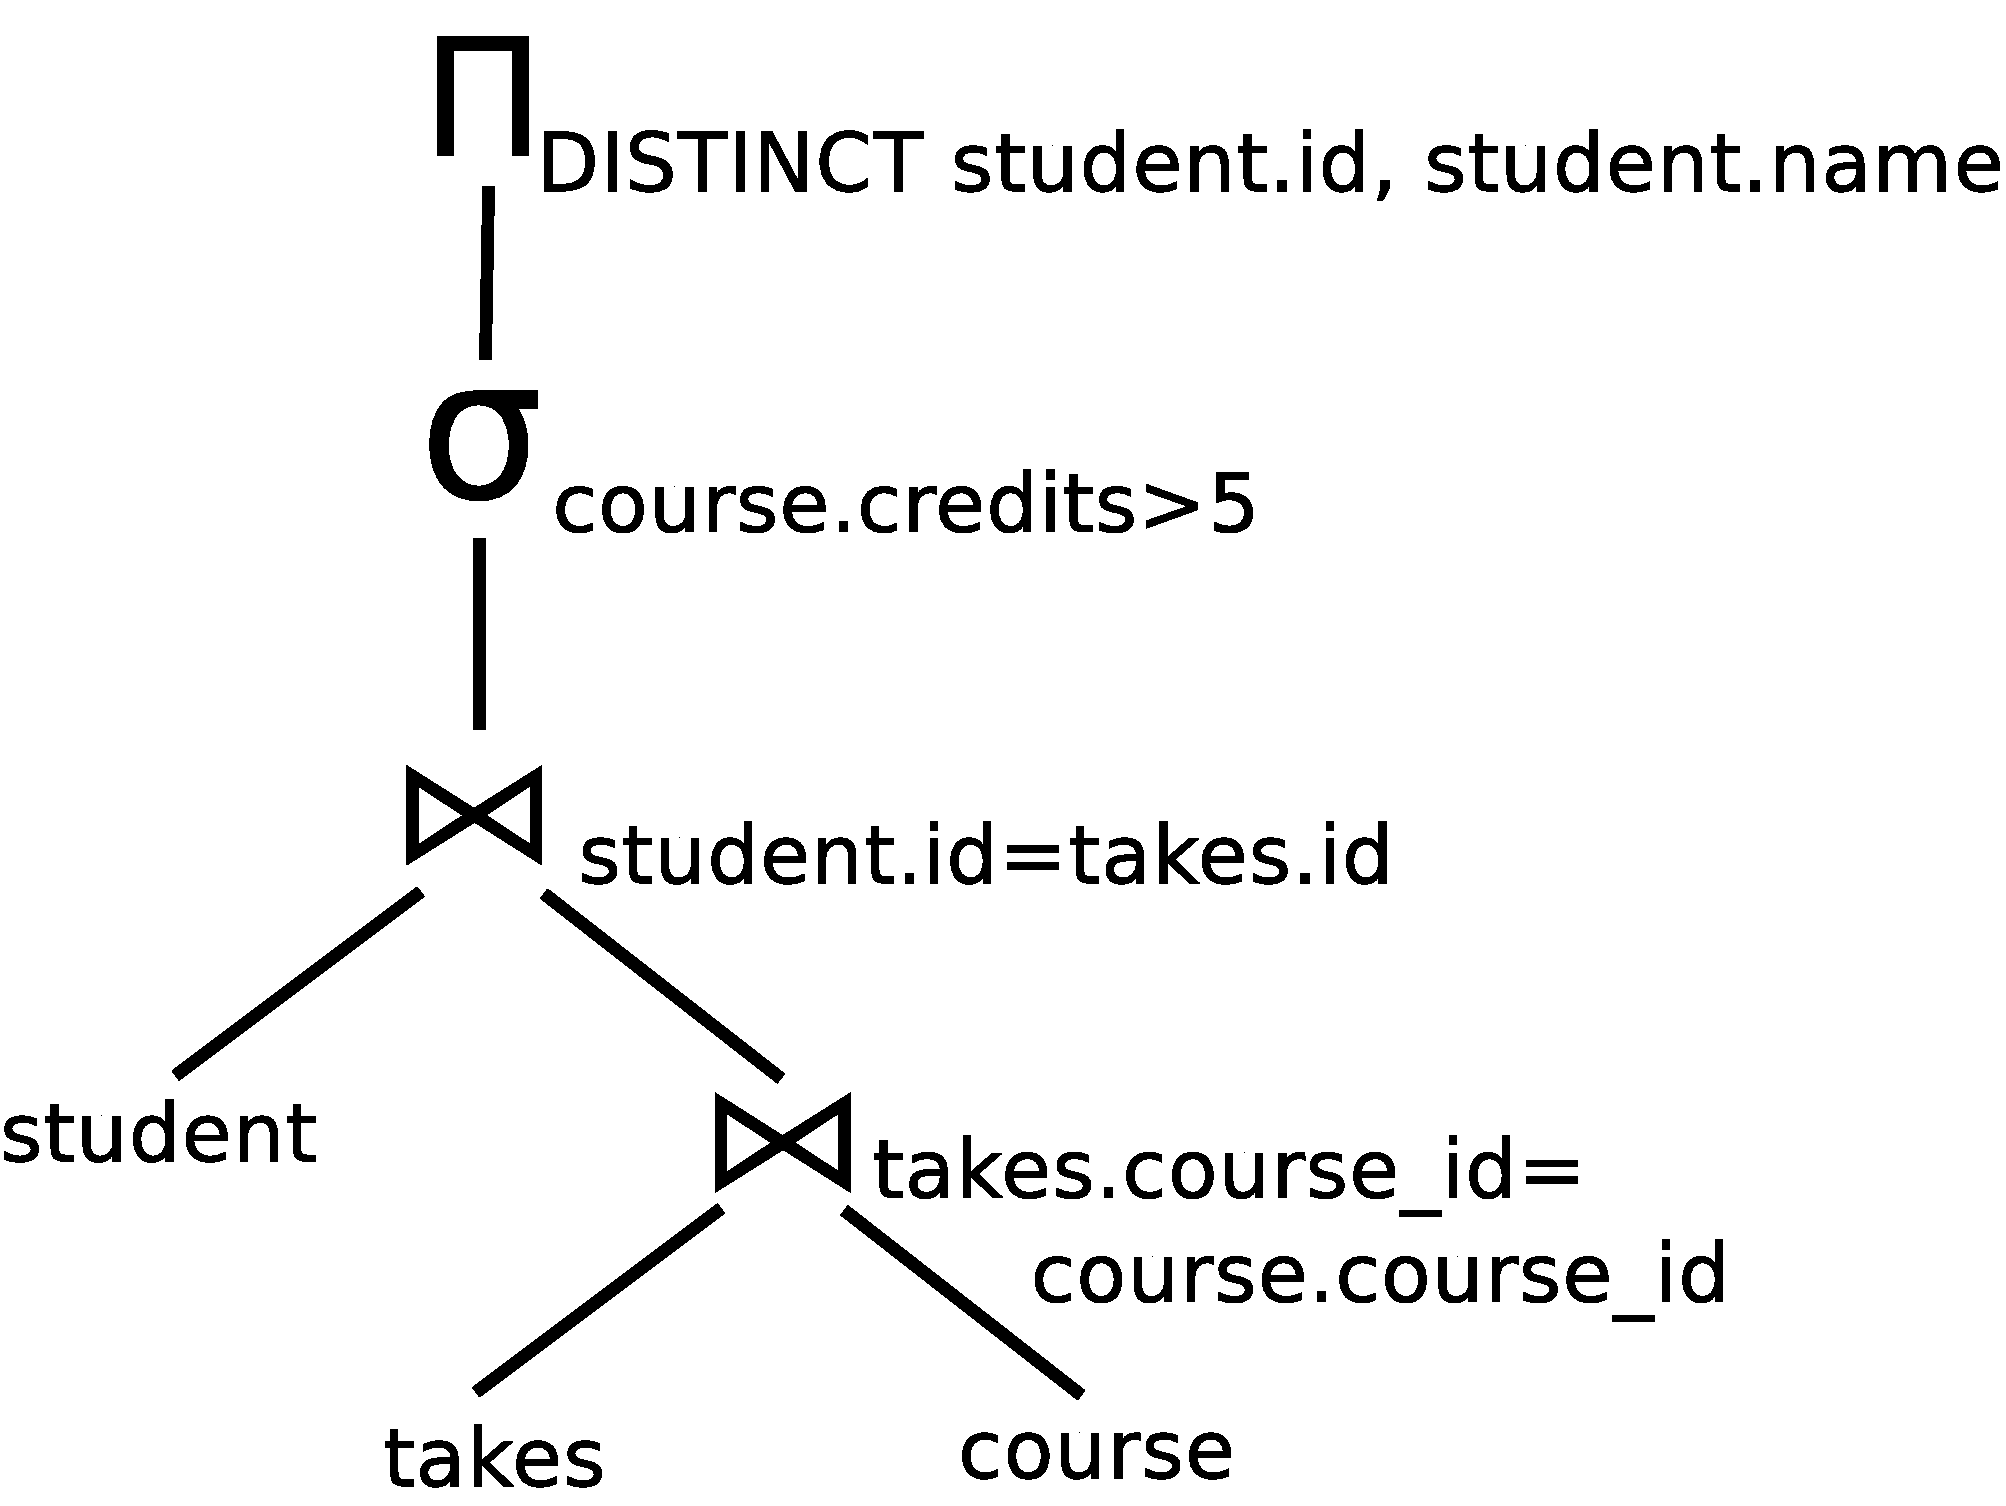
\includegraphics[width=1\textwidth,keepaspectratio=true]{/parsedTree.pdf}
		\caption{Parsed Tree From Query}
		\label{fig:parsedTree}
	\end{minipage}
		\begin{minipage}{0.59\textwidth}
	\centering
	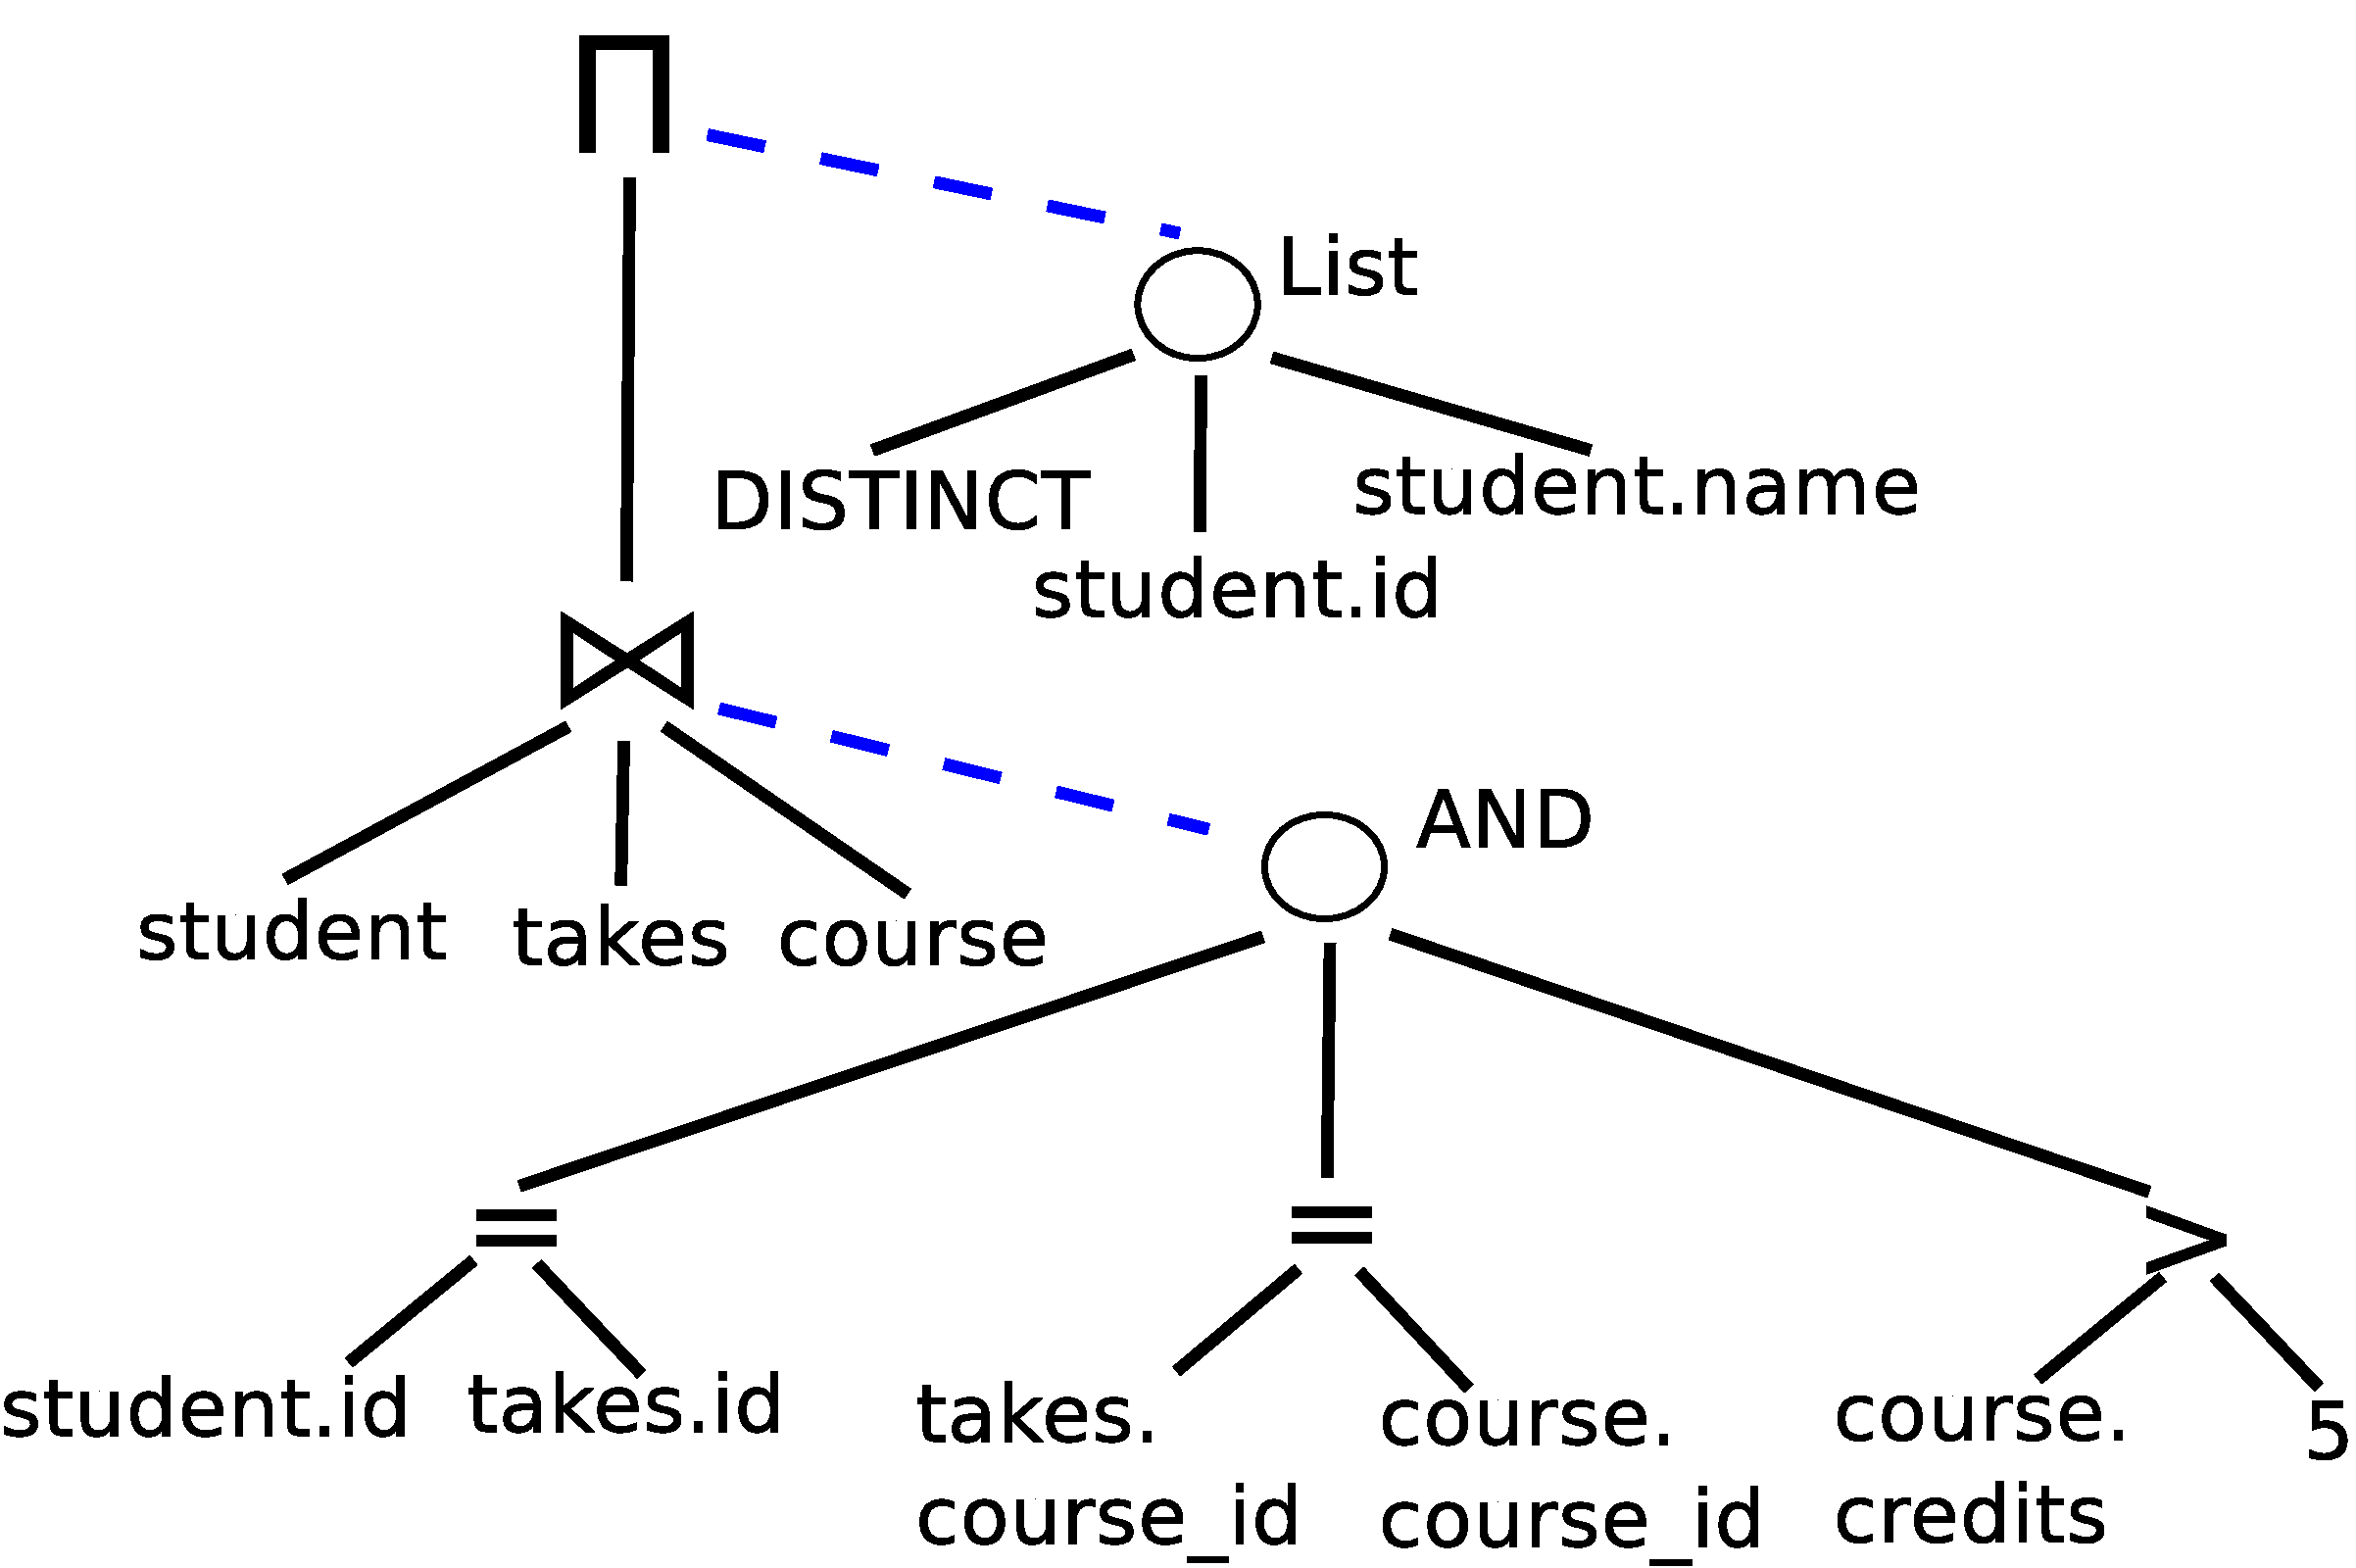
\includegraphics[width=1\textwidth,keepaspectratio=true]{/flattenedTree.pdf}
		\caption{Flattened Tree}
		\label{fig:flattenedTree}
	\end{minipage}
\end{figure}


\subsection{Edit Sequence Based Grading}
XData considers the following form of edits to the flattened tree generated from the student query.
\begin{itemize}
    \item  inserting a node/subtree into the flattened tree
\item removing a node/subtree from the flattened tree
\item replacing an existing node/subtree from a flattened tree
with another node/subtree in the flattened tree
\item moving a node/subtree from one position of the flattened
tree to another
\end{itemize}

When editing a flattened tree generated from a student query, an infinite number of possible edits could be made. However only edits that make the query more similar to the correct query would be useful. In order to add edits that make the student query more similar to the correct query, XData uses the correct query to guide the edits that are generated. The guided edits are based on the differences the student flattened student query tree has with the flattened tree of the correct query. For example, query attributes/conditions/constructs not used in the correct query but present in the student query will be removed when generating edits. 
For each query edit that XData generates, marks corresponding to the edit as configured by the instructor are deducted. The marks deducted for the edit can be considered the edit cost. 

XData can generate multiple guided edits on the student query at each step. From each of these edited queries, more edits are possible. Consider a graph whose nodes are all queries for the given schema. For a student query  SQ, edits of the query are also nodes in the graph. Let these edited queries be connected to query SQ with an edge whose weight is the edit cost of the edited query. Canonically equivalent queries, i.e. their canonical forms are the same, are connected by 0 cost edges. The sequence of edits that has the least cumulative cost can now be determined based on the shortest path in this graph from the student query node in the graph to a correct query node. Partial marks can now be awarded based on this shortest path.  Since the weight of each edge, which represents the cost of edit is non-negative, the shortest possible path may be found using Dijkstra’s shortest path algorithm. Hence, given a set of edits and using a given set of canonicalizations, the shortest path in the graph, as defined above, gives the edit sequence with the least cost.  
We note that the graph discussed above is for the ease of understanding only and XData does not proactively try to generate the entire graph. In practice, XData generates the nodes of the graph on the fly as needed. 

In case the instructor specifies multiple correct queries, the edit sequence based algorithm run based on all correct queries and the best partial marks obtained is awarded. 

\subsection{Heuristic solution}
Even with using only guided edits, the search space is still very large for larger queries if we consider all guided edits to get the shortest path from the student query to the correct query. Hence in practice, we use a greedy heuristic. The heuristic uses a cost benefit model. For each  edited query we can get an estimate of how incorrect the query is by finding the differences between the canonicalized versions of the edited query and the correct query. A weighted sum (based on the weight assigned by the instructor for each edit) can be used to find an edit distance which we call the \textit{canonicalized edit distance}. Each guided edit reduces the canonicalized edit distance to the correct query. The reduction in the canonicalized edit distance from the edit is the benefit of the edit. 

For the heuristic algorithm, at each edit step, we find the $benefit-cost$ for each edit. We then pick the edit that has the highest value of the $benefit-cost$ and use it to generate further edits. The remaining edits are discarded at each step. Using the heuristic allows XData to search a much smaller search space. For the incorrect student queries that we had in our course, we found that the heuristic solution works as well and takes orders of magnitude less time as compared to the exhaustive solution  \cite{xdata:comad}.



\section{Automated Grading Experience}
\label{sec:exp}
We have successfully used the XData automated grading system across several offerings of undergraduate database courses at IIT Bombay. Before using XData in a course, we empirically confirmed, using results from a previous database course, that XData was able to catch as many as or more errors than when the grading was done manually or when fixed datasets are used for grading. This result was consistent across all questions that XData was able to grade. We found, in several cases, that manual grading had missed subtle errors such as a missing distinct clause. 

For the initial course offerings, we used only generated dataset based grading to check for correctness and had to award partial marks manually. The dataset-based grading significantly reduced the human effort involved and allowed us to catch more errors than would have been possible with manual grading.
In several cases, however, students were not satisfied since they could not intuitively understand how marks had been deducted or what the error in their specific query was. The tagged datasets on which the student queries failed were shown but often there would be too many of them to understand the specific error. A dataset designed to catch one type of mutation may catch other types of mutations as well and hence it was not always clear what the actual error was. Several students contested the scores that they had been awarded when their query was found to be incorrect. Awarding partial marks manually by the graders was still tedious since students often wrote queries in very different and complex ways. Manually transforming such student queries to a simpler form was difficult. For instance, in one case a correct query involved using a NOT IN clause and some students used a combination of multiple EXCEPT and INTERSECT clauses.  

When using partial marking in combination with dataset based evaluation, we reduced the human effort as well as provided much better feedback. 
We experienced fewer students contest grades when it was assigned automatically compared to when a human would manually assign grades. The edit-based guidance was also  useful for students to understand where they went wrong. For the first course setting where we used automated partial marking for evaluation, we found that across 1800 student query submissions that were graded by XData, only 2 queries were contested by students. In both cases, we traced back the errors in grade to bugs in our code. One of the main challenges when using automated grading was to provide sufficient types of correct queries that covered the student queries.  

Since the edit sequence based guided edits provide a way to change an incorrect student query to a correct query, the guided edits can be used by students to learn the mistakes that they made and how the mistakes could have been corrected. Such feedback was very helpful especially for beginners to understand how to write correct SQL queries.  